\section{Motivation}
\label{sec:motivation}

\subsection{Threat Model}%
\label{sub:threat_model}

Sultan \etal~\cite{sultan2019_container_security} propose four broad categories of container-related threats. \Cref{fig:threat_model} presents an overview of each category. An application running within a container might attack the container itself, attempting to escape confinement or interfere with the execution of co-located applications running within the same container. Inter-container threats are similarly possible, wherein one container attempts to interfere with or take over another. Since containers share the underlying host operating system, it is also possible for a container to directly attack the host, either by escaping confinement altogether or by launching denial of service or resource consumption attacks. Finally, a malicious or semi-honest host system may attack containers running within it. Researchers have generally recognized that mitigating this fourth category of attack requires the use of hardware security mechanisms \cite{sultan2019_container_security} \todo{cite others} such as trusted execution environments or trusted platform modules. Such host-to-container attacks are, therefore, out of scope for this paper.

\begin{figure}[htpb]
  \centering
  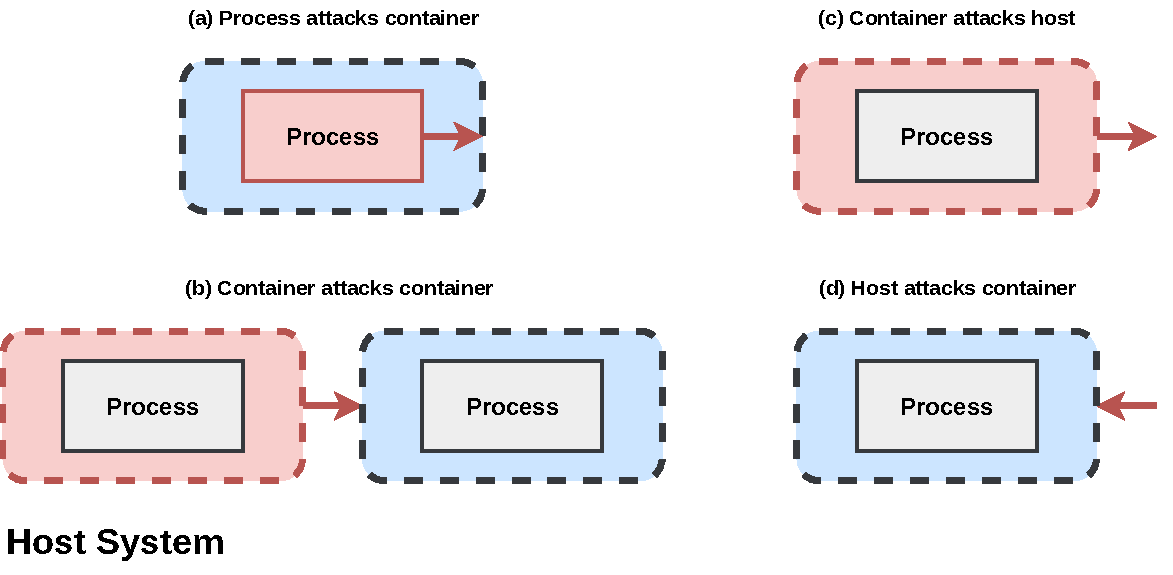
\includegraphics[width=0.8\linewidth]{figs/threat-model.pdf}
  \caption{
    Four categories of container-related attacks \cite{sultan2019_container_security}. \textbf{(a)} A process running within a container attacks the container itself. \textbf{(b)} One container attacks another container. \textbf{(c)} A container attacks the host system. \textbf{(d)} The host system attacks the container. This fourth category of attack is out of scope for this paper.
  }%
  \label{fig:threat_model}
\end{figure}

In this threat model we consider three broad classes of attack vector, comprised of the containers and the applications that run within them. These attack vectors are described in turn below.
\begin{enumerate}[label=\bfseries AV\arabic*., ref=AV\arabic*, labelindent=1em]
  \item \textsc{Malicious Applications.}
    A malicious application is designed with express malicious intent. Malicious software may actively attempt to subvert other applications, other containers, or the host system itself. This subversion could include privilege escalation attacks on the host system, denial of service attacks on other containers or the host, or the installation of backdoors. A sophisticated attacker could even abuse a malicious application to install a rootkit \cite{beegle2007_rootkit} in the container, on the host system, or in the host's firmware, stealthily gaining permanent and possibly overprivileged access.
  \item \textsc{Semi-Honest Applications.}
    In contrast with malicious applications, semi-honest applications are not necessarily expressly designed with malicious intent and might even be cooperative with other applications or containers. However, the semi-honest application can passively participate in unwanted activity, such as surveillance or consumption of the host's resources.
  \item \textsc{Vulnerable Applications.}
    Vulnerable applications running inside containers may become compromised by attackers, often with the goal of using these applications to orchestrate a more sophisticated attack on other applications running within the same container, other containers, or the host system itself \cite{sultan2019_container_security}. Common vulnerabilities here include code execution vulnerabilities on untrusted input, memory corruption bugs, and privilege escalation vulnerabilities in a container's configuration. Exploitation of kernel-level vulnerabilities are also a concern here, as an attacker can potentially abuse a legitimate application to target vulnerable code paths in the kernel \cite{xin2018_container_security}.
\end{enumerate}

Since containers are often co-located in large-scale, multi-tenant systems such as the cloud \cite{sultan2019_container_security}, the potential for exploitation or abuse by foreign threat actors is exacerbated. Thus, it is imperative that container management systems enforce least-privilege on containers to prevent such exploitation from negatively impacting the rest of the system.

\subsection{The Quest for Secure Containers}%
\label{sub:secure_containers}

\subsection{Why an eBPF Implementation?}%
\label{sub:why_ebpf}

\todo{
\begin{itemize}
  \item Can be dynamically loaded without rebooting the kernel
  \item Guaranteed safety
  \item Can be used in production without downtime
  \item Container-specific LSM $\rightarrow$ Only apply policy to a given container
  \item Dynamically instrument non-lsm functions in the kernel, such as \texttt{commit\_creds}, this allows us to prevent kernel privilege escalation attacks like the ones described in Xin \etal~\cite{xin2018_container_security}
\end{itemize}
}
